\documentclass[fleqn,a4paper,20pt]{article}
 \usepackage{amstext}
 \usepackage[pdftex]{graphicx}
\usepackage[bottom=2.5cm, right=1.5cm, left=1.5cm, top=2.5cm]{geometry}
 \usepackage[english]{babel}
% \usepackage {boekF}
\setlength{\parindent}{0pt}
\usepackage{xcolor}
\usepackage{epstopdf}
\usepackage[utf8]{inputenc}
\usepackage[justification=centering]{caption}

\usepackage{amsmath,mathtools,amssymb}%ss
\usepackage[arrow]{hhtensor}



 \graphicspath{ {./images/} } 
\begin{document}


\begin{center}
$\ $\\

	
{\Huge \textbf{ TOMAS User Guide}}

\vspace{3.0cm}

\begin{figure}[h!]
	\centering
	\includegraphics[width=\linewidth]{TOMAS1}
\end{figure}


\vspace{3.0cm}
\end{center}

\begin{flushright}{by J. Buermans (2024)} \end{flushright}

\newpage
%%%%%%%%%%%%%%%%%%%%%%%%%%%%%%
\section{TOMAS main systems}%%	
%%%%%%%%%%%%%%%%%%%%%%%%%%%%%%


\subsection{Main Equipment Rack}

\begin{figure}[h!]
	\centering
	\includegraphics[width=\linewidth]{MainRack1}
\end{figure}


\newpage
\subsection{Cooling system}

\begin{figure}[h!]
	\centering
	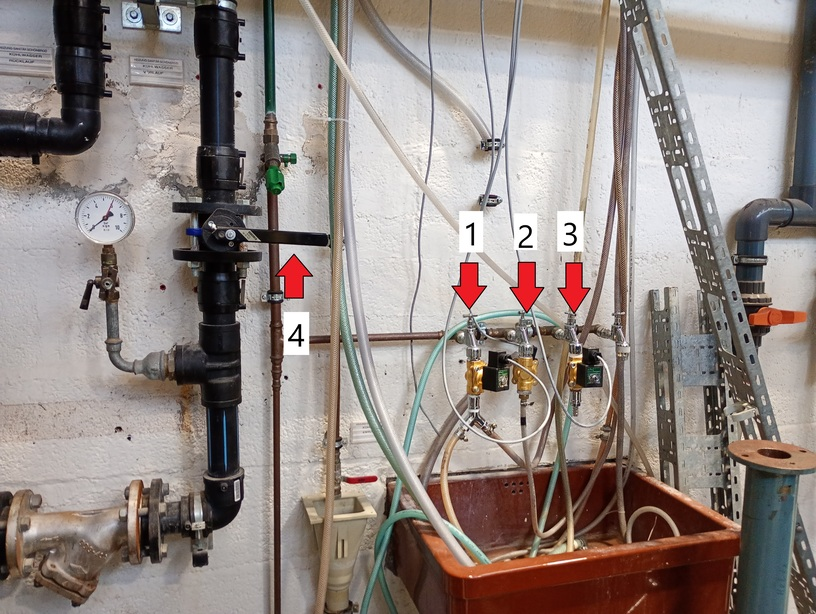
\includegraphics[width=\linewidth]{Cool2}
\end{figure}

\begin{enumerate}
	\item Cooling EC source and window
	\item Cooling turbopump
	\item Not in use
	\item Main valve Cooling for magnets
\end{enumerate}

\newpage
%%%%%%%%%%%%%%%%%%%%%%%%%%%%
\section{Before operation}%%	
%%%%%%%%%%%%%%%%%%%%%%%%%%%%


Before operating TOMAS, some safety checks should be performed.

\subsection{Vacuum}

\begin{minipage}{.68\textwidth}
	
The average neutral pressure is shown on the readout unit located in the main equipment rack.	The vacuum vessel pressure is shown on the Channel 1 (upper number) of the readout. To start an operation the pressure level should be $\approx 5\cdot 10^{-7}$ mbar. If the pressure is slightly higher check that calibration of the Channel 1 is set for N2 (air). In other cases, check the Troubleshooting.\\

\textcolor{red}{\textbf{Before starting any plasma operation, check the pressure in the vacuum vessel.}}\\

The gas injection system is located in a large support structure close to one of the tangential ports of the vacuum vessel. The gas injection system has 4 mass flow controllers directly connected to helium, hydrogen, argon and deuterium bottles.\\

\textcolor{red}{\textbf{Check that the gas bottles are closed.}}\\

The upstream and downstream pipes of the gas injection system must be evacuated from the residual gas prior an injection start.
\end{minipage}
\begin{minipage}{.02\textwidth}
	$\ $\\
\end{minipage}
\begin{minipage}{.3\textwidth}
	\centering
	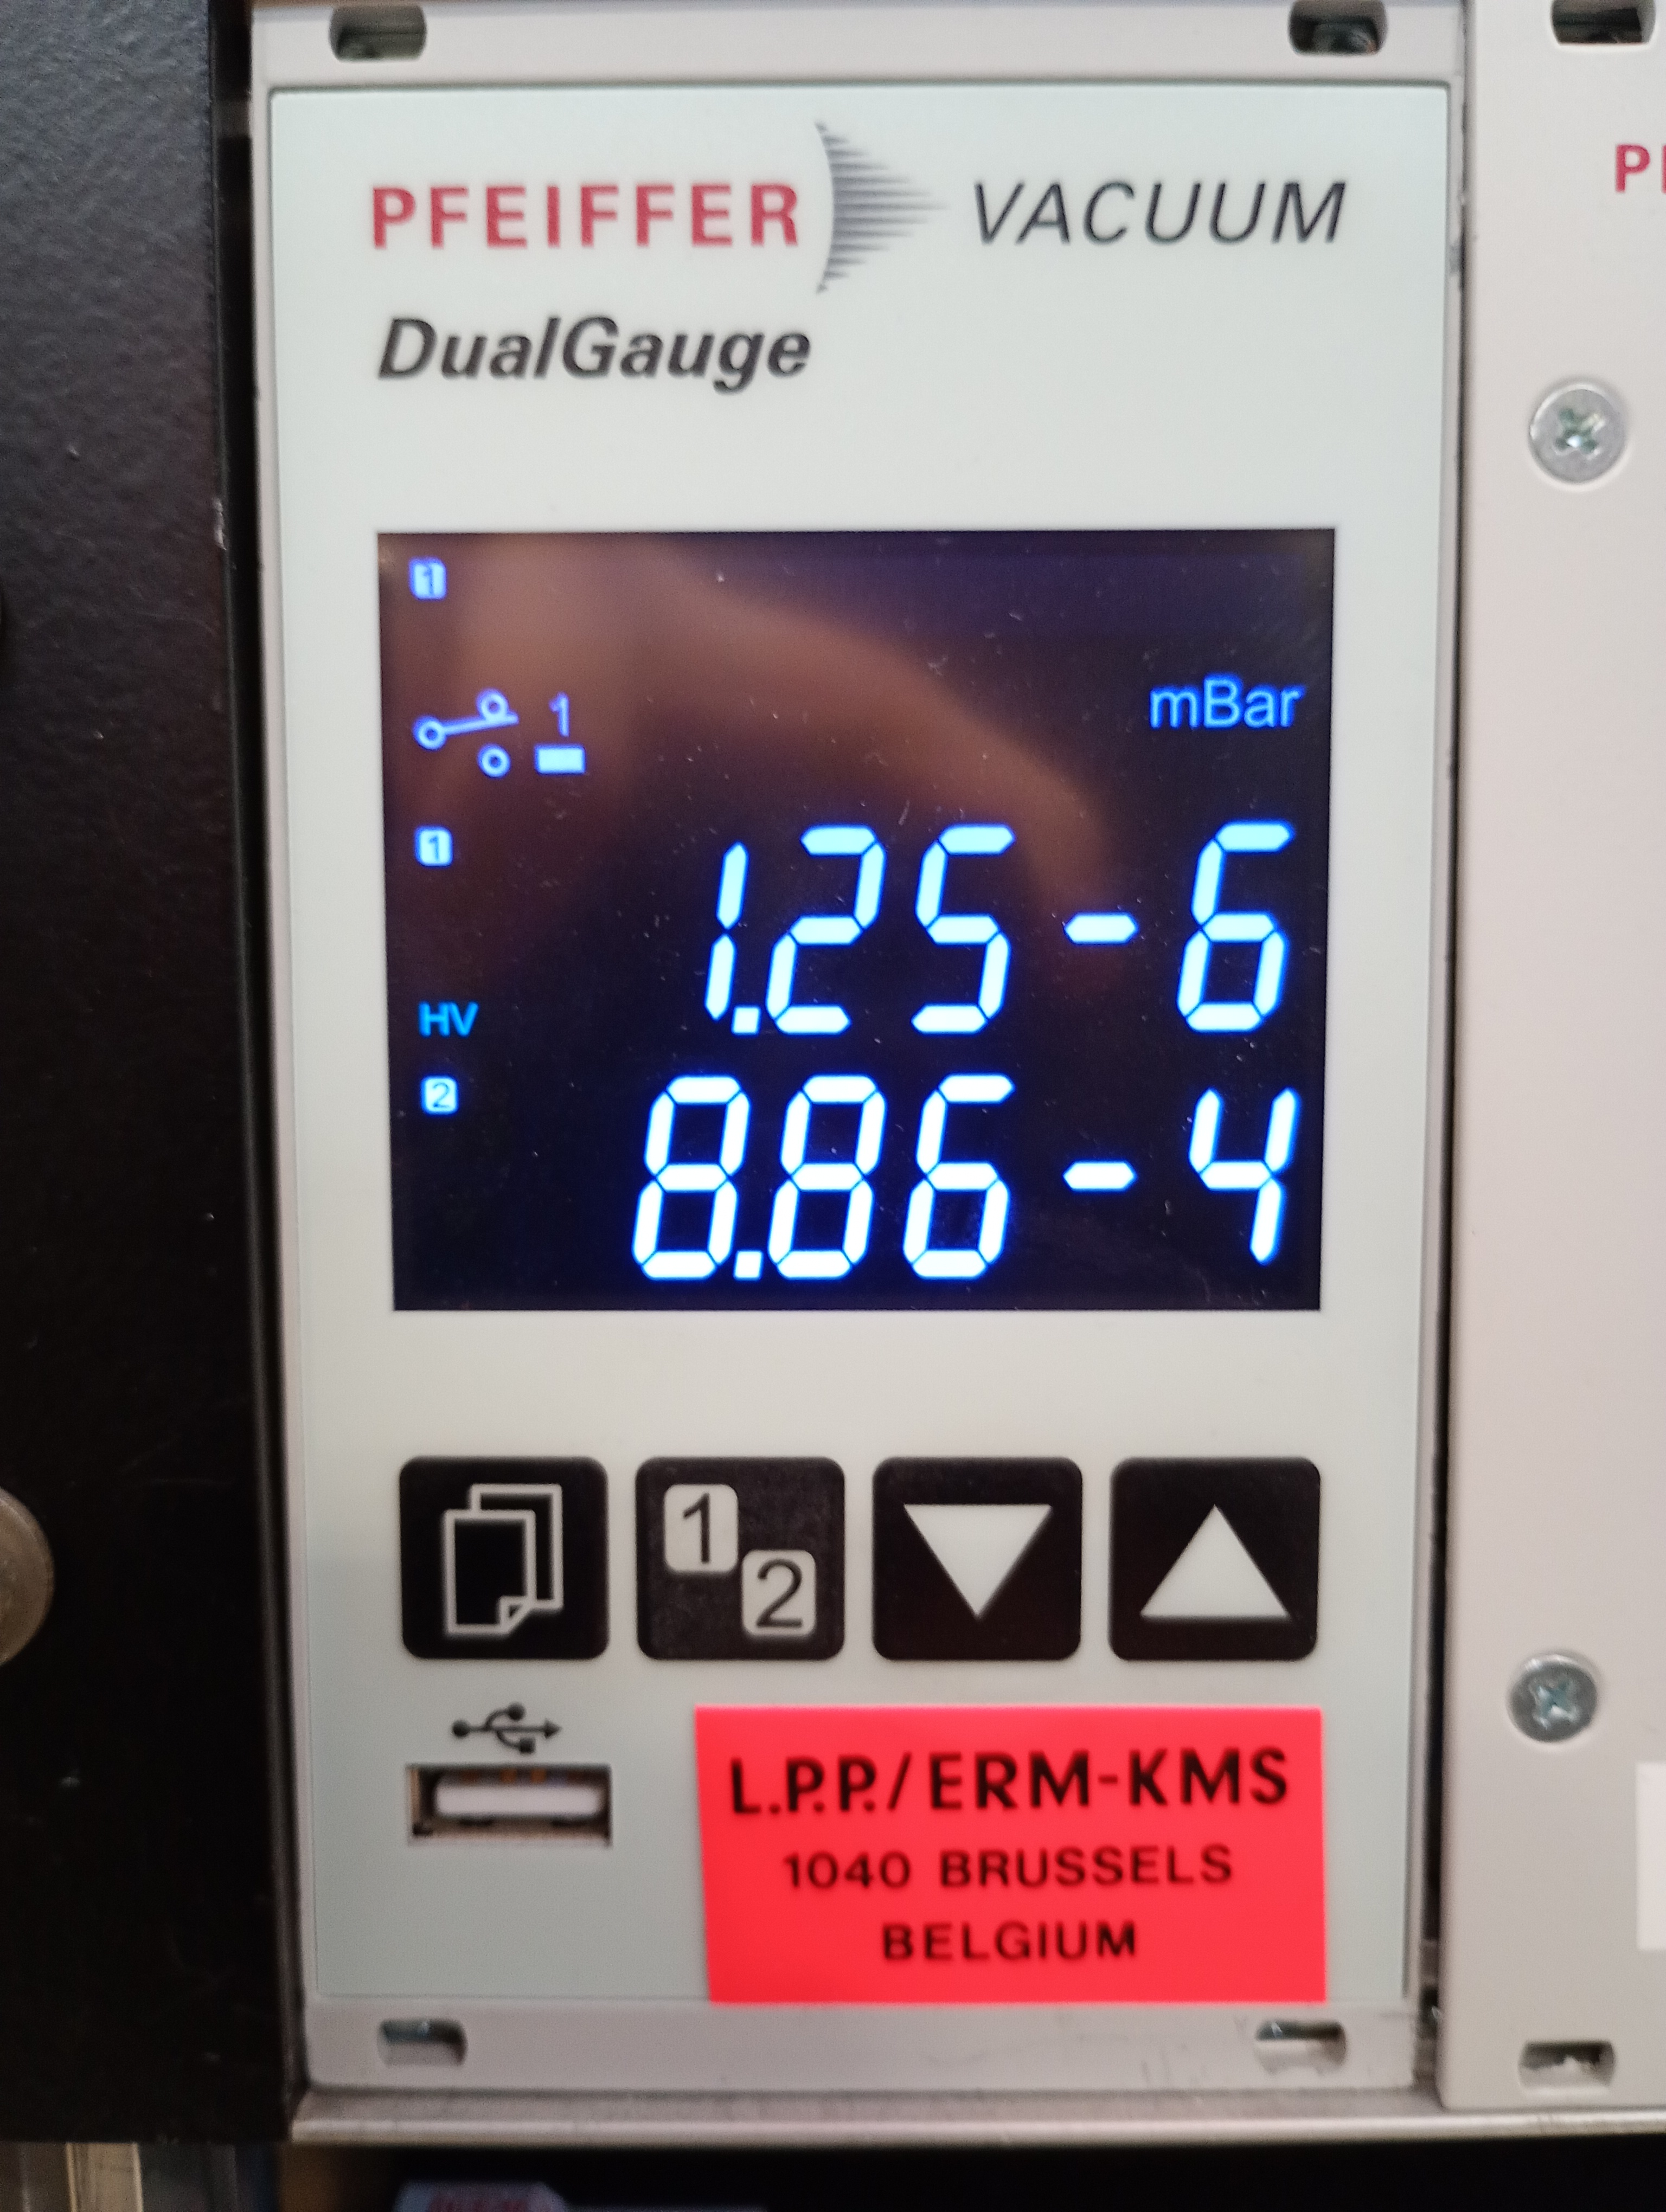
\includegraphics[width=\linewidth]{Pressure1}
\end{minipage}


\vspace{0.5cm}
Find the small metallic valves below the mass flow controllers (Figure \ref{Gas1} (1)). If any element above a valve is missing don’t open a corresponding valve! \\

\textcolor{red}{\textbf{Open the small metallic valves located below each mass flow controller (Figure \ref{Gas1} (1)).}}\\

Open the `\textit{Flowmeter}' tab in the Control System and go to the section \textbf{Pressure Control} the activate the `\textit{Forpump Flowmeter}' (Figure \ref{Gas2}).\\


\textcolor{red}{\textbf{Activate the Forepump to clear the lines (Figure \ref{Gas2}).}}\\

\begin{minipage}{.3\textwidth}
	
{Check if the vacuum pump connected to the upstream pipes is switched on. Pump down the upstream pipes during 10 – 15 minutes. }\\

{
	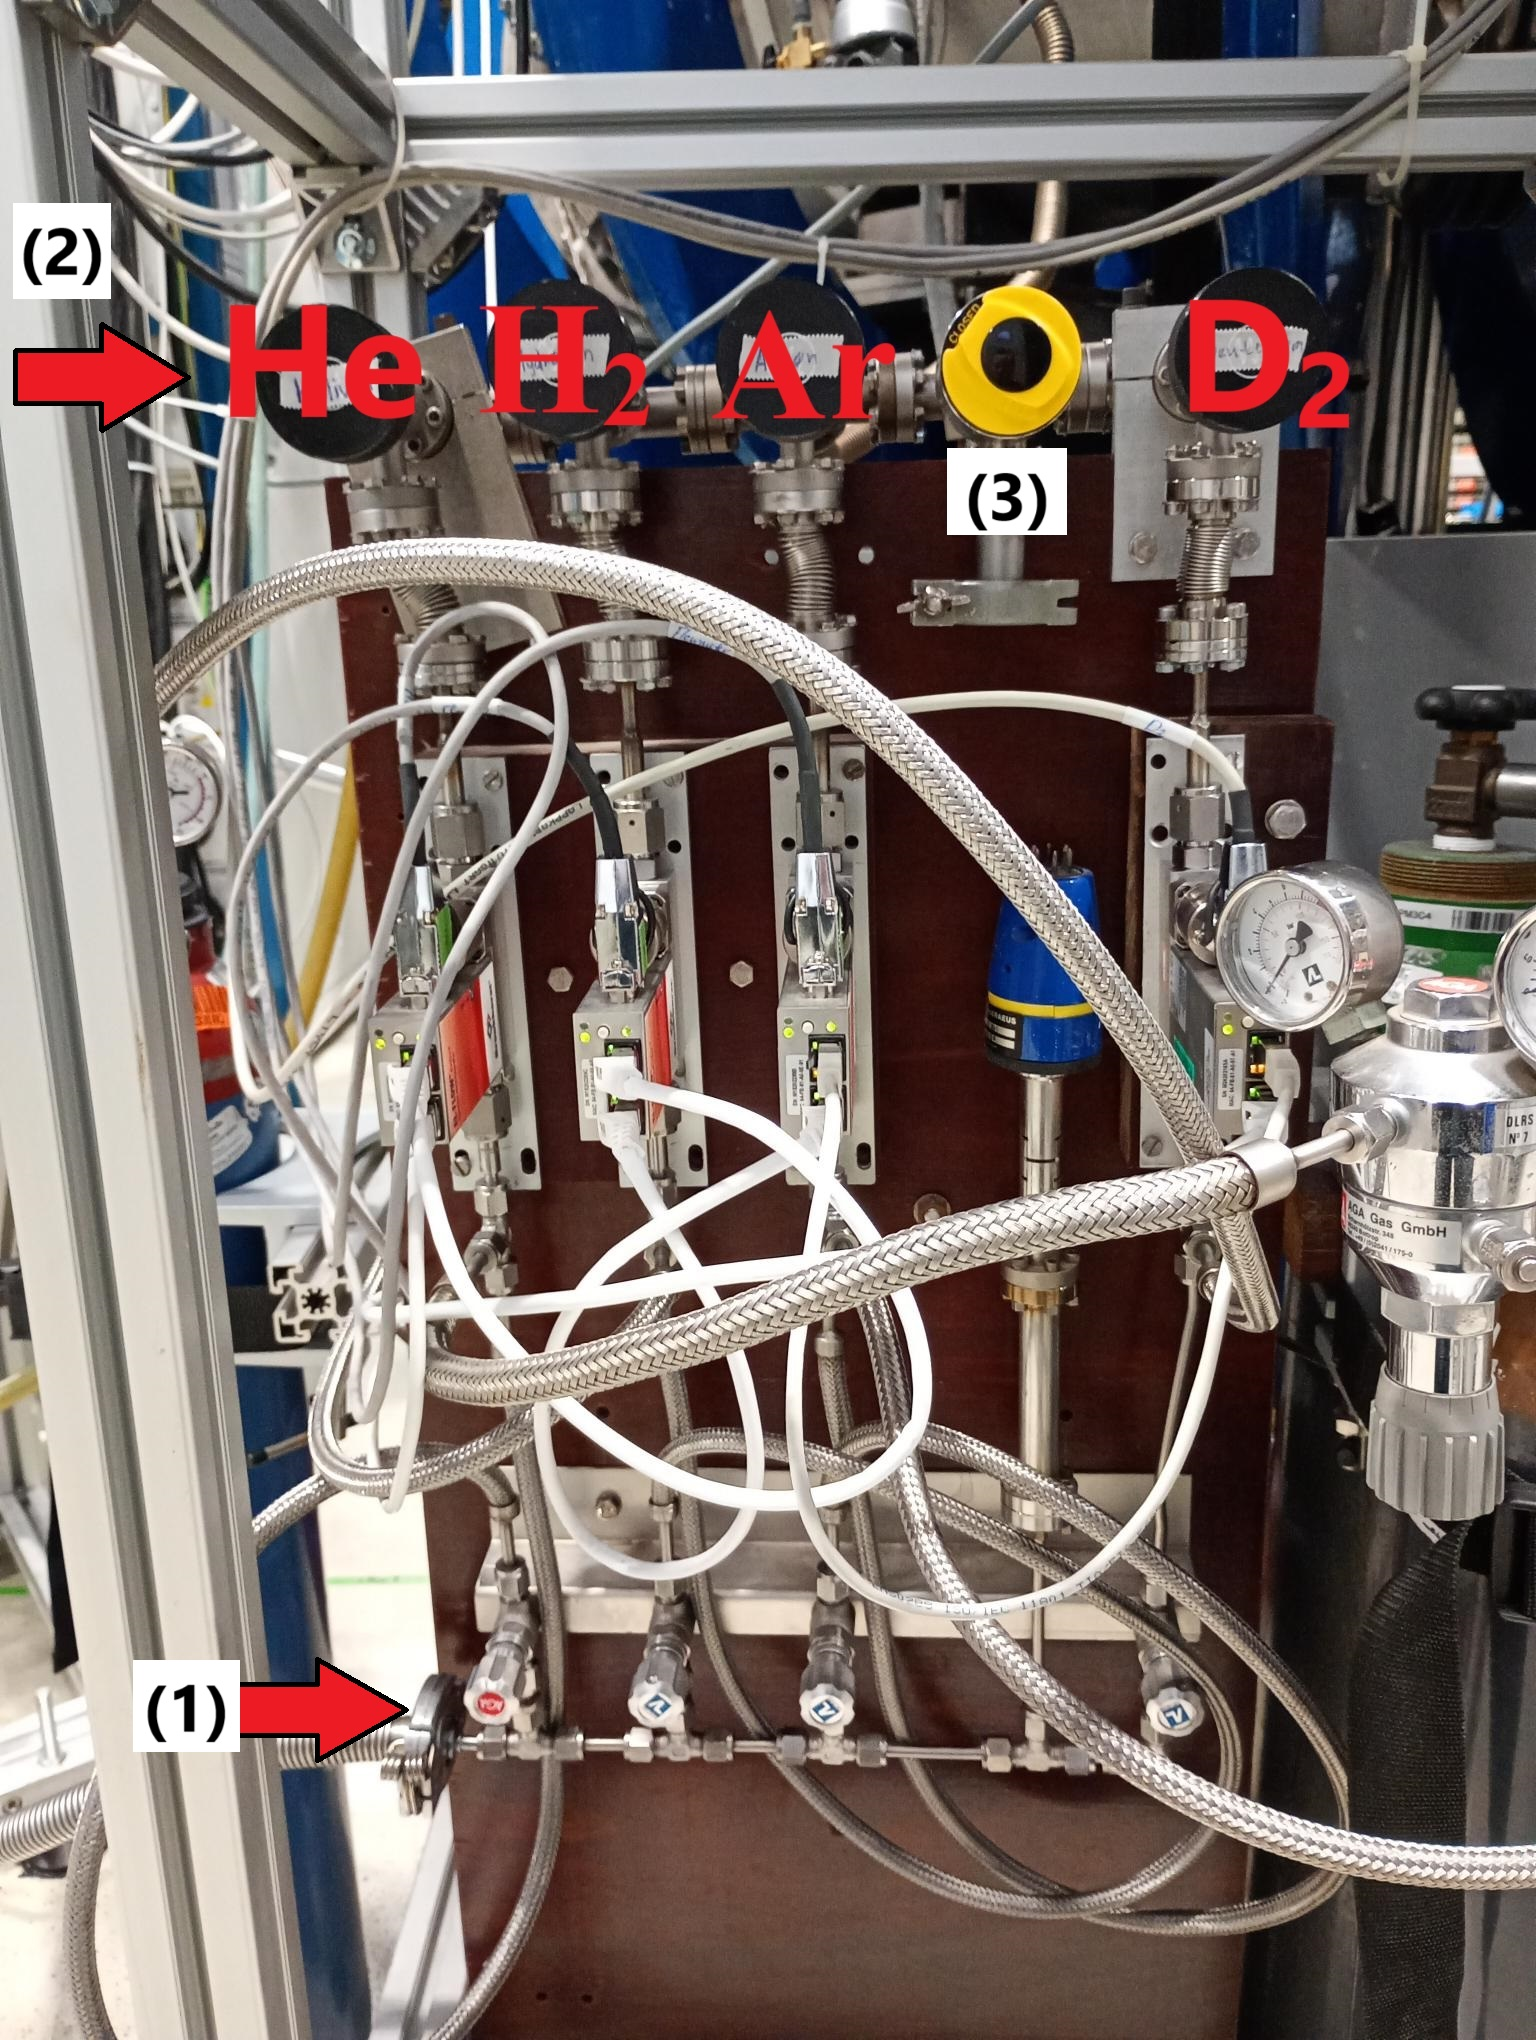
\includegraphics[width=\linewidth]{Gas1}
	\captionof{figure}{The gas injection system}
	\label{Gas1}}
\end{minipage}
\begin{minipage}{.02\textwidth}
	$\ $\\
\end{minipage}
\begin{minipage}{.68\textwidth}
	\centering
	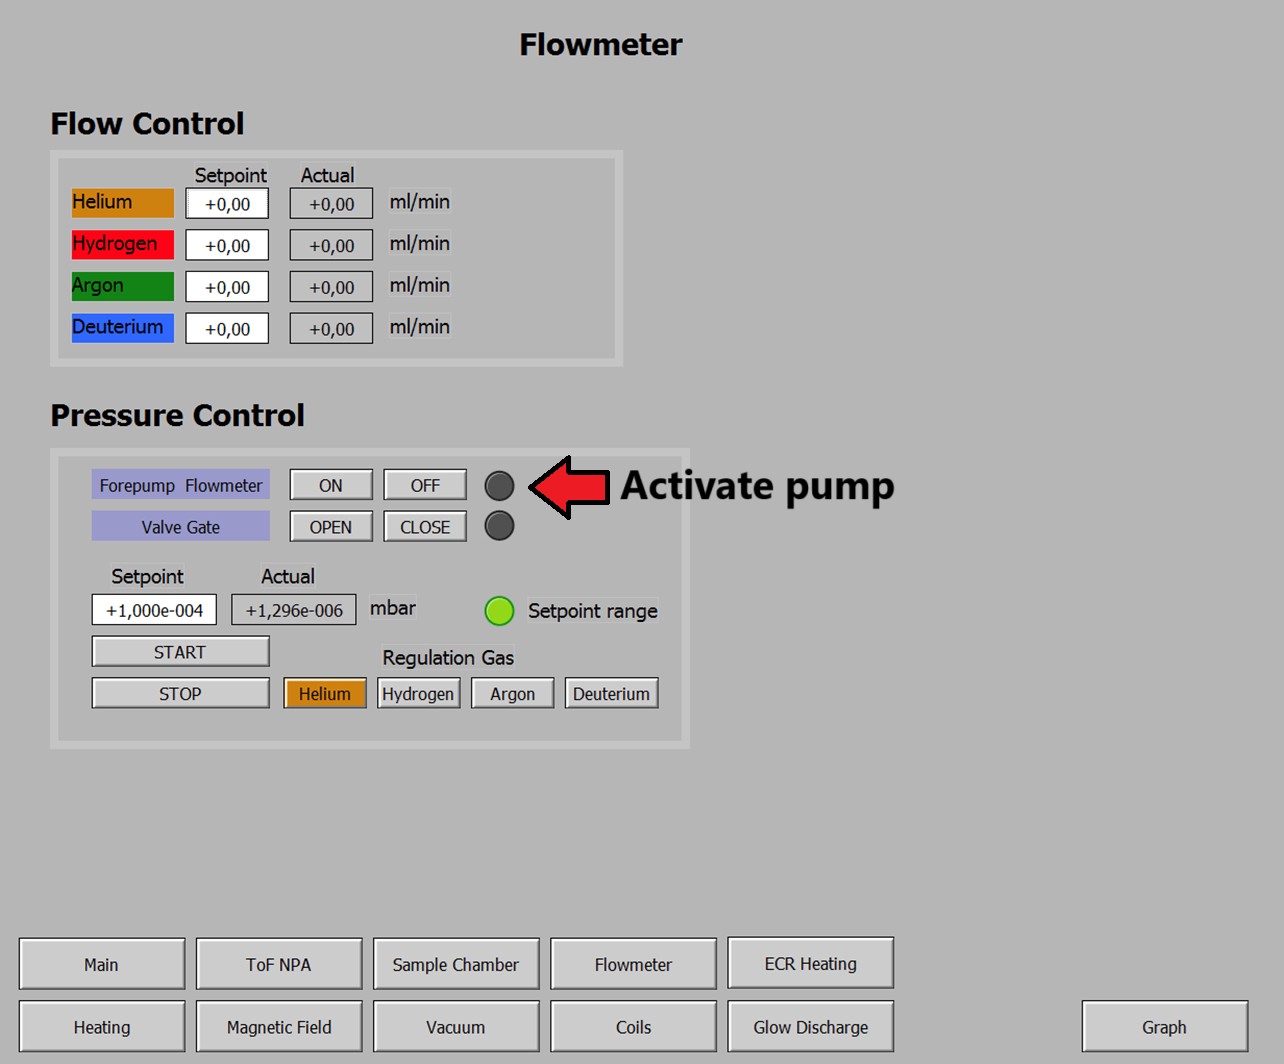
\includegraphics[width=0.95\linewidth]{Gas2}
	\captionof{figure}{The `\textit{Flowmeter}' tab in the Control System}
	\label{Gas2}
 
\end{minipage}	
	
\newpage
\textcolor{red}{\textbf{Close all small metallic valves and deactivate the Forepump.}}\\
		
\textcolor{red}{\textbf{Open the needed bottle(s).}}\\

Check that both manometers on the gas reducer connected to each bottle shows a pressure different from 0. Otherwise, check the Troubleshooting.\\

\textcolor{red}{\textbf{Open the respective black valves above the mass flow controller(s) (Figure \ref{Gas1} (2)).}}\\


Don’t open the yellow valve (Figure \ref{Gas1} (3)). This is used to vent the machine. Check that the black shutter connecting the gas injection system to the tangential port is open (downward position). Since no gas is injected yet, the pressure level should not change significantly. If needed, wait until the pressure level is back at  $\approx 5\cdot 10^{-7}$ mbar. 

		
	
\newpage
\subsection{Cooling}

The cooling system for the cooling of the coils, the turbo-pump, the EC source and the EC window is activated automatically by the control system. However, the main valve for the cooling of the coils, needs to be opened manually. Change the position of the black lever arm from horizontal to $30^\circ$ (Figures \ref{Cool4}-\ref{Cool5}). Position changing requires pushing the lever arm interlock. Verify that the water pump for the closed water circuit is activated (black button on Figure \ref{Cool9}).\\

For safe operation, the electrical resistance of the cooling water has to be high enough to avoid that the coil current flows through the cooling water. This can be checked on the conductance meter (Leitwertmesser) (Figure \ref{Cool9}). The distillatory pump  is activated automatically when the coil current is switched on.\\

\begin{minipage}{.5\textwidth}
	\centering
	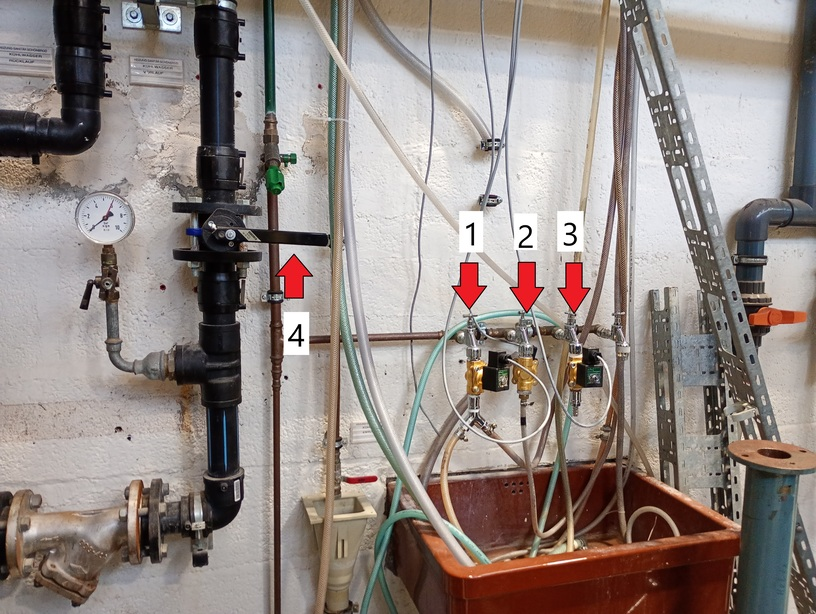
\includegraphics[width=0.95\linewidth]{Cool2}
	\captionof{figure}{Cooling systems with \textbf{1.}Cooling for EC source and window \textbf{2.}Cooling for turbopump \textbf{3.}Not in use \textbf{4.}Main valve for cooling of the coils}
	\label{Cool2}
	\begin{minipage}{.49\textwidth}
		\centering
		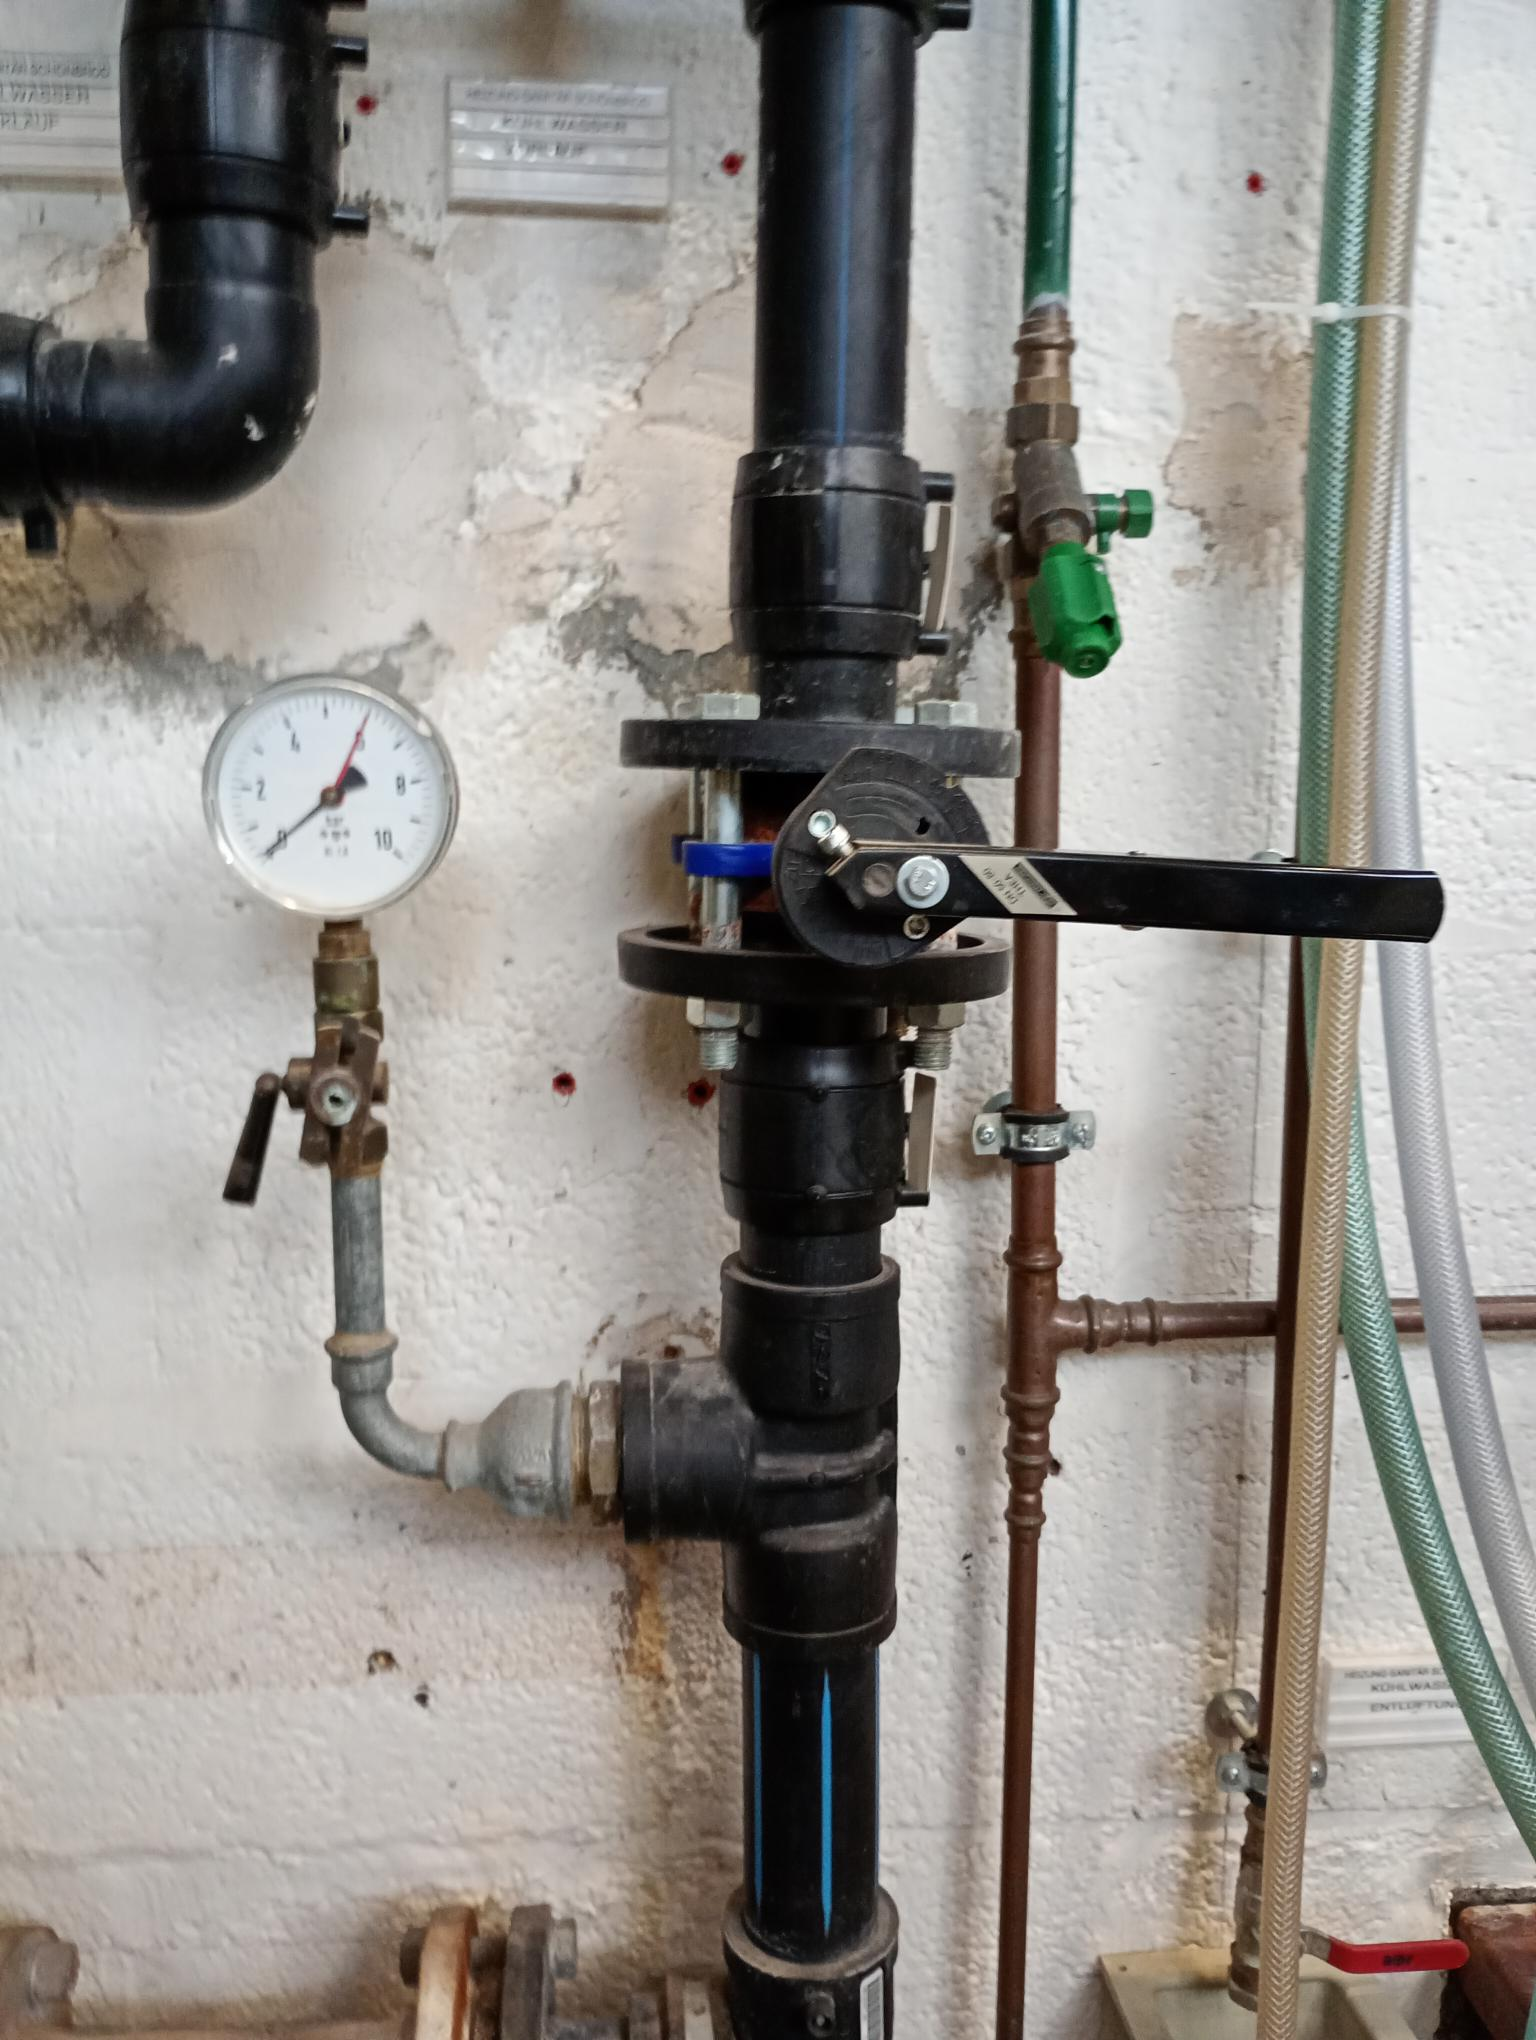
\includegraphics[width=0.95\linewidth]{Cool4}
		\captionof{figure}{Coils cooling off}
		\captionsetup{width=.2\textwidth}
		\label{Cool4}
	\end{minipage}
	\begin{minipage}{.49\textwidth}
		\centering
		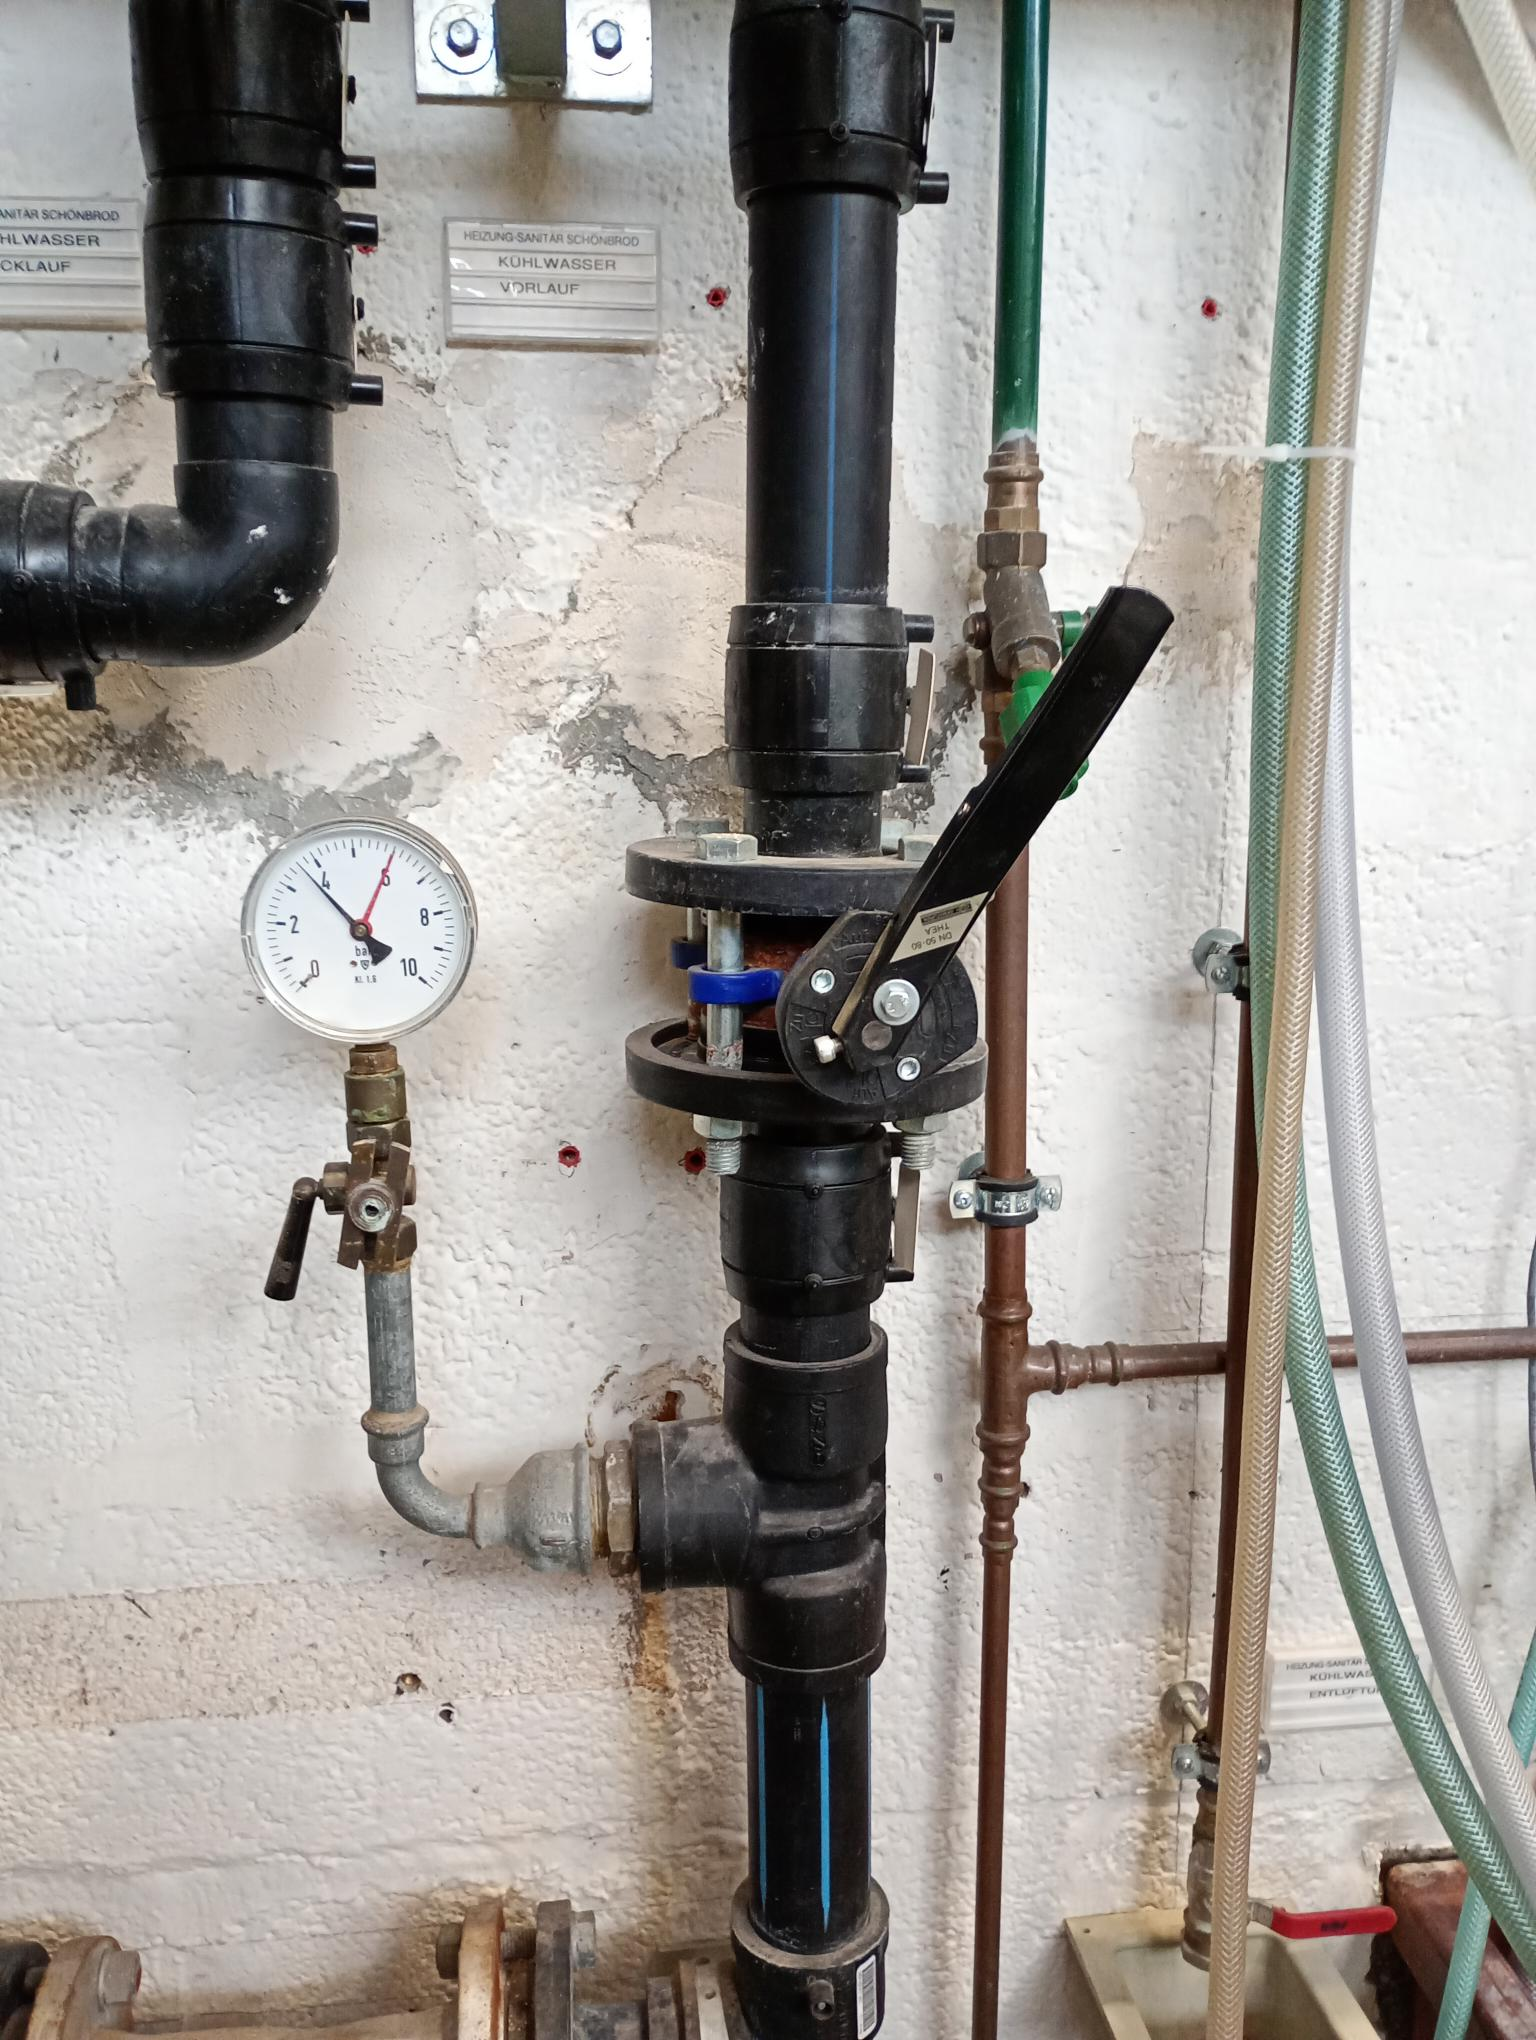
\includegraphics[width=0.95\linewidth]{Cool5}
		\captionof{figure}{Coils cooling on}
		\label{Cool5}
	\end{minipage}
\end{minipage}
\begin{minipage}{.5\textwidth}
	\centering
	\includegraphics[width=0.95\linewidth]{Cool9}
	\captionof{figure}{Closed water circuit pump with power switch (right) and conductance meter (bottom)}
	\label{Cool9}
	\vspace*{0.9cm}
\end{minipage}



\vspace*{0.5cm}


\begin{minipage}{.5\textwidth}



\end{minipage}

%The wave equation can be written as:
%\begin{equation}
%\left[ \left( \omega^2 - c^2 k^2\right)  \matr{e} + c^2 \vec{k}\cdot \vec{k}\right] \cdot \vec{E_1}= \dfrac{1}{\epsilon_0} i\omega \vec{J_1}
%\end{equation}
%To find a solution $\vec{E_1}(\vec{r},t)$ for this wave equation (dispersion relation) we need to eliminate $\vec{J_1}$. Taking into account possible boundary conditions, we can find a relation between $\vec{J_1}$ and $\vec{E_1}$ : $\vec{J_1} = \matr{\sigma}\cdot\vec{E_1}$, where $\matr{\sigma}$ is the conductivity tensor.\\
%
%For a cold electron plasma, where there is no acoustic coupling and collisions with ions are neglected, we find: $i\omega \vec{J_1}=\epsilon_0\omega^2_p\vec{E_1}$ with the plasma frequency $\omega^2_{pe} = n_eq^2_e/m_e\epsilon_0$ . The quantity $\epsilon_0\omega^2_p/i\omega$ plays the role of complex conductivity. The wave equation reduces to:
%\begin{equation} \left[ \left( \omega^2 - c^2 k^2-\omega^2_p\right)   \matr{e} + c^2 \vec{k}\cdot \vec{k}\right] \cdot \vec{E_1}= \vec{0}\end{equation}
%
%A wave is longitudinal if $\vec{E_1} \parallel \vec{k}$. This wave is always electrostatic. There is no oscillating magnetic field since $\vec{k} \times \vec{E_1}=\omega \vec{B_1}=\vec{0}$. Since $ \vec{k}\cdot \vec{k} \cdot \vec{E_1}=k^2\vec{E_1}$, the dispersion relation reduces to $\omega^2=\omega^2_{pe}$. These are the well-known local plasma oscillations that do not propagate in the plasma.\\
%
%A wave is transversal if $\vec{E_1} \perp \vec{k}$. With $\vec{E_1}$ a vector $\vec{B_1}$ is associated:  $\vec{k} \times \vec{E_1}=\omega \vec{B_1}$. This wave is always electromagnetic, since with the oscillating electric field an oscillating magnetic field is associated with amplitude $B_1=kE_1/\omega$. Since $ \vec{k}\cdot \vec{k} \cdot \vec{E_1}=\vec{0}$, the dispersion relation becomes $\omega^2=c^2k^2+\omega^2_{pe}$.\\
%
%The plasma is dispersive and has a refractive index and a dielectric constant: $n^2=c^2k^2/\omega^2=\epsilon_r=1-\omega^2_{pe}/\omega^2$.
%\begin{itemize}
%	\item With $\omega < \omega_{pe}$ correspond imaginary values of $k$ and there is no wave propagation $(n<0)$.
%	\item With $\omega = \omega_{pe}$ corresponds a cut-off.
%	\item For $\omega > \omega_{pe}$, real values of $k$ exist and the wave can propagate undamped through the plasma.
%\end{itemize}
%
%As a wave propagates into a plasma several different phenomena can occur with respect to the deposition of its wave energy: reflection, transmission, absorption and mode conversion. An incident wave is in general partially reflected and partially transmitted.\\

%\textbf{Reflection} For an outside launch the wave sees an increasing density as it propagates towards the centre. It also sees a slightly increasing magnetic field because of the $1/R$ dependence. As it reaches a zone where it cannot propagate, the wave reflects back. At this point $k\rightarrow0, n\rightarrow0$ and we reach a cut-off.\\
%
%\textbf{Transmission} If the evanescent region is small (with respect to the wavelength) the wave can partially tunnel through this region.\\
%
%\textbf{Absorption} A strong wave-particle resonance can occur leading to a strong absorption. This is the case where $k\rightarrow\infty$. The resonance occurs when the parallel Doppler shifted frequency is equal to an exact harmonic of the cyclotron frequency: $\omega = k_\parallel v_\parallel+\ell \omega_{ce}$. 
%\begin{itemize}
%	\item $\ell=0$: Landau damping
%	\item $\ell=0$: Fundamental frequency heating
%	\item $\ell=0$: Second harmonic heating
%\end{itemize}
%
%\textbf{Mode conversion} This involves two different plasma waves. the wave encounters a wave resonance which mode converts it into a different type of plasma wave. Again $k\rightarrow\infty$. Some of the energy of the incident wave is transferred to the second wave which propagates further into the plasma.\\
%
%In a magnetized plasma the Lorentz force also acts on the charge carriers. We neglect electron-ion collisions and the acoustic coupling. The presence of an external magnetic field $\vec{B_0}$ introduces an electron cyclotron frequency $\omega_{ce} = -q_eB_0/m_e$. This magneto-plasma behaves as a circularly birefringent medium. We obtain two dispersion relations and two different waves can be distinguished. 
%
%\begin{itemize}
%	\item \textbf{Ordinary wave} (O-wave) or L-circularly polarized wave.
%		\begin{equation}
%		\omega^2=c^2k^2+\dfrac{\omega^2_{pe}\omega}{\omega + \omega_{ce}}
%		\end{equation}
%	\item \textbf{Extraordinary wave} (X-wave) or R-circularly polarized wave.
%		\begin{equation}
%		\omega^2=c^2k^2+\dfrac{\omega^2_{pe}\omega}{\omega - \omega_{ce}}
%		\end{equation}
%\end{itemize}
%
%\newpage
%%%%%%%%%%%%%%%%%%%%%%%%%%%%%
%\section{Ordinary wave}%%%%%
%%%%%%%%%%%%%%%%%%%%%%%%%%%%%%%%%%%%
%\subsection{O-mode Accessibility}%%
%
%The ordinary wave has a component of the electric field parallel to the background magnetic field: $E_{\parallel}\neq0$. The rotation is opposite to that of the cyclotron rotation of the electron. The O-mode dispersion equation becomes:
%	\begin{equation}
%	n_\perp^2=K_\parallel=1-\dfrac{\omega_{pe}^2}{\omega^2}-\dfrac{\omega_{pi}^2}{\omega^2}\approx 1-\dfrac{\omega_{pe}^2}{\omega^2}
%	\end{equation}
%
%The O-wave can only propagate for $\omega > \omega_{pe}$. For typical TOMAS parameters ($B_0 = 90 \ mT$) this leads to a cut-off density for the O-mode of $7.87e16\ m^{-3}$.
%
%%%%%%%%%%%%%%%%%%%%%%%%%%%%%%%%%
%\subsection{O-mode absorption}%%
%
%The heating efficiency for O-mode absorption can be written as $\eta_h=1-e^{-\lambda_O}$ with:
%	\begin{equation}
%	\lambda_O =\dfrac{\pi}{4}\cdot \dfrac{v_{T_e}^2}{c^2}\cdot \dfrac{\omega_{ce}R_0}{c}\dfrac{\omega_{pe}^2}{\omega_{ce}^2}\cdot \sqrt{1-\dfrac{\omega_{pe}^2}{\omega_{ce}^2}}
%	\end{equation}
%
%With $v_{T_e} = \sqrt{\dfrac{k\cdot T_e}{m_e}}=$ electron thermal velocity.\\
%
%For the TOMAS-device, O-wave absorption is very small. At $10 \ eV$ only $0.025 \% $ can be absorbed at an ideal density close to $ 5.25e16 \ m^{-3}$. With a ECRF power source of $2\ kW$ (supposedly only emitting O-wave polarization) only $0.5\ W$ can be coupled to the plasma with a single pass.
%\begin{figure}[!h]
%	\centering
%	\includegraphics[width=\linewidth]{AbsorptionOwaveTOMAS}
%	\caption{Absorption of the O-wave at the Electron Cyclotron Resonance layer in TOMAS for $B_0 = 90 \ mT$}
%	\label{fig:AbsorptionOwaveTOMAS}
%\end{figure}
%
%\newpage
%If the value of the magnetic field is raised, O-wave absorption also rises, moving the electron cyclotron resonance layer from the High Filed side (HFS) to the Low Field Side (LFS). The O-wave cut-off is consequently raised. The influence is rather small. 
%
%\begin{figure}[!h]
%	\centering
%	\includegraphics[width=\linewidth]{AbsorptionOwaveTOMASBsweep}
%	\caption{Absorption of the O-wave at the Electron Cyclotron Resonance layer in TOMAS for $T_e = 10 \ eV$}
%	\label{fig:AbsorptionOwaveTOMASBsweep}
%\end{figure}
%
%
%
%%%%%%%%%%%%%%%%%%%%%%%%%%%%%%%
%\section{Extraordinary wave}%%
%%%%%%%%%%%%%%%%%%%%%%%%%%%%%%%
%\subsection{Accessibility}%%
%
%
%The extraordinary wave has no component of the electric field parallel to the background magnetic field: $E_{\parallel}=0$. The rotation corresponds with the cyclotron rotation of the electrons. We get a different solution for the dispersion equation: 
%\begin{equation}
%n_\perp^2=\dfrac{\left( \omega^2+\omega\omega_{ce}-\omega_{pe}^2 \right)\cdot \left( \omega^2-\omega\omega_{ce}-\omega_{pe}^2 \right) }{\omega^2 \cdot \left( \omega^2-\omega_{ce}^2-\omega_{pe}^2 \right)}
%\end{equation}
%
%
%
%This equation leads to four domains: 2 where wave propagation is possible and 2 evanescent regions (Figure	\ref{fig:XFreqDomain} and \ref{fig:XDensDomain}). Three interesting values for the frequency $\omega$ can be identified:
%\begin{itemize}
%	\item \textbf{R cut-off:} The Fast X-wave (FX) can propagate if $\omega>\omega_R$. For typical TOMAS parameters ($B_0 = 90 \ mT$) this leads to a cut-off density for the FX-mode of $2.11e15\ m^{-3}$.
%		\begin{equation}
%		\omega_R=\dfrac{\omega_{ce}+\sqrt{\omega_{ce}^2+4\omega_{pe}^2}}{2} 
%		\end{equation}
%	\item \textbf{L cut-off:} The Slow X-wave (SX) can propagate if $\omega>\omega_L$. For typical TOMAS parameters ($B_0 = 90 \ mT$) this leads to a cut-off density for the SX-mode of $1.51e17\ m^{-3}$.
%		\begin{equation}
%		\omega_L=\dfrac{-\omega_{ce}+\sqrt{\omega_{ce}^2+4\omega_{pe}^2}}{2} 
%		\end{equation}
%	\item \textbf{Upper Hybrid Resonance (UHR):} A wave resonance occurs for $\omega=\omega_{UHR}$. For typical TOMAS parameters ($B_0 = 90 \ mT$) this occurs at a density of $8.06e15\ m^{-3}$.
%		\begin{equation}
%		\omega_{UHR}= \sqrt{\omega_{pe}^2+\omega_{ce}^2}
%		\end{equation}
%\end{itemize}
%
%\paragraph{Conclusion} In TOMAS X-mode heating  at the fundamental harmonic is not possible because the wave cannot propagate if the density exceeds $2e15\ m^{-3}$.
%
%\begin{figure}[!h]
%	\centering
%	\includegraphics[width=\linewidth]{XFreqDomain}
%	\caption{TOMAS X-wave accessibility domains ($B_0=90 mT, n_e = 5e16 m^{-3}$)}
%	\label{fig:XFreqDomain}
%\end{figure}
%\begin{figure}[!h]
%	\centering
%	\includegraphics[width=0.78\linewidth]{XDensDomain}
%	\caption{TOMAS X-wave density domains ($B_0=90 mT$)}
%	\label{fig:XDensDomain}
%\end{figure}
%
%When we consider second harmonic heating, the situation improves considerably. If we want the ECR-layer to remain at the same position, the toroidal magnetic field has to be halved ($B_0 = 45 \ mT$). Again four regions can be determined regarding the density:
%\begin{itemize}
%	\item \textbf{R cut-off:} The Fast X2-wave (FX2) can propagate if the density stays below $3.94e16\ m^{-3}$.
%	\item \textbf{L cut-off:} The Slow X2-wave (SX2) can propagate if the density stays below $1.18e17\ m^{-3}$.
%	\item \textbf{Upper Hybrid Resonance (UHR):} A wave resonance occurs at a density of $5.90e16\ m^{-3}$.
%\end{itemize}
%
%\begin{figure}[!h]
%	\centering
%	\includegraphics[width=0.78\linewidth]{X2DensDomain}
%	\caption{TOMAS X2-wave density domains ($B_0=45 mT$)}
%	\label{fig:X2DensDomain}
%\end{figure}
%
%%%%%%%%%%%%%%%%%%%%%%%%%%%%%%%%%%
%\subsection{X1-mode absorption}%%
%
%The heating efficiency for X1-mode absorption can be written as $\eta_h=1-e^{-\lambda_X}$ with:
%\begin{equation}
%\lambda_X =\dfrac{1}{2}\pi\cdot \dfrac{v_{T_e}^2}{c^2}\cdot \dfrac{\omega_{ce}R_0}{c} \cdot \alpha(2-\alpha)^{5/2}\cdot (1+\sqrt{\alpha})
%\end{equation}
%
%With $\alpha =\dfrac{\omega_{pe}^2}{\omega_{ce}^2} $.\\
%
%
%For the TOMAS-device, X1-wave absorption is very small. At $10 \ eV$ only $0.0215 \% $ can be absorbed close to the R cut-off density of $ 2.11e15 \ m^{-3}$. With a ECRF power source of $2\ kW$ (supposedly only emitting X-wave polarization) only $0.43\ W$ can be coupled to the plasma with a single pass. This is comparable to the O-wave absorption, but only applicable at very low density.\\
%
%If we can manage to introduce the Slow X-wave (SX) into the plasma core, the absorption efficiency can raise to $0.313 \%$  at an ideal density close to  $ 5.18e16 \ m^{-3}$. This can only be achieved using a HFS launch or by mode conversion.
%
%
%
%\begin{figure}[!h]
%	\centering
%	\includegraphics[width=0.91\linewidth]{AbsorptionXwaveTOMAS}
%	\caption{Absorption of the X-wave at the Electron Cyclotron Resonance layer in TOMAS for $B_0 = 90 \ mT$}
%	\label{fig:AbsorptionXwaveTOMAS}
%\end{figure}
%
%%%%%%%%%%%%%%%%%%%%%%%%%%%%%%%%%%
%\subsection{X2-mode absorption}%%
%
%The heating efficiency for X2-mode absorption can be written as $\eta_h=1-e^{-\lambda_{X2}}$ with:
%\begin{equation}
%\lambda_{X2} =2\pi\cdot \dfrac{v_{T_e}^2}{c^2}\cdot \dfrac{\omega_{ce}R_0}{c} \cdot \dfrac{\alpha(2-\alpha)^{1/2}(6-\alpha)^{5/2}}{32(3-\alpha)^{5/2}}
%\end{equation}
%
%%With $\alpha =\dfrac{\omega_{pe}^2}{\omega_{ce}^2} $.\\
%
%For the TOMAS-device, X2-wave absorption is small. At $10 \ eV$ only $0.147 \% $ can be absorbed at an ideal density close to $ 3.44e16 \ m^{-3}$. With a ECRF power source of $2\ kW$ (supposedly only emitting X-wave polarization) only $2.94\ W$ can be coupled to the plasma with a single pass.
%
%\begin{figure}[!h]
%	\centering
%	\includegraphics[width=0.91\linewidth]{AbsorptionX2waveTOMAS}
%	\caption{Absorption of the X2-wave at the Electron Cyclotron Resonance layer in TOMAS for $B_0 = 45 \ mT$}
%	\label{fig:AbsorptionX2waveTOMAS}
%\end{figure}
%
%\newpage
%
%%%%%%%%%%%%%%%%%%%%%%%%%%
%\subsection{Comparison}%%
%
%
%Second harmonic X2-mode heating ($0,147 \%$) is more than 5 times more effective than O-mode heating ($0,025 \%$), but has a lower cut-off density. Fundamental X-mode heating is most efficient, up to $0.31\%$, but the FX-wave can only reach the plasma core when it is launched from the HFS. Launching from the LFS limits the accessibility to a density of $2.11e15\ m^{-3}$.
%
%\begin{figure}[!h]
%	\centering
%	\includegraphics[width=\linewidth]{AbsorptionOXX}
%	\caption{Comparison of O-wave and X-wave absorption}
%	\label{fig:AbsorptionOXX}
%\end{figure}
%
%It is clear that fundamental X-mode heating can only be used at very low densities in the TOMAS device. Single pass absorption leads to a maximum coupling of $0.43\ W$, which is extremely low and seems insufficient for plasma production. Second harmonic X-mode heating couples three times less power with respect to fundamental heating. O-mode absorption is even 10 times lower with respect to fundamental heating. We can conclude that single pass absorption of O-wave or X-wave isn't likely to produce a plasma in the TOMAS device. Other mechanisms should be investigated to determine how a plasma can be produced:
%
%\begin{itemize}
%	\item Multiple passes of the X-wave after reflection on the vessel wall can increase absorption efficiency. For the fundamental mode, the R cut-off still limits the density to $2.11e15\ m^{-3}$. This mechanism can perhaps initiate plasma production.
%	\item Multiple passes of the O-wave after reflection on the vessel wall can increase absorption efficiency. This mechanism can perhaps contribute to the initial plasma production and the density build-up beyond the R cut-off. Efficiency stays limited.
%	\item Mode conversion.
%\end{itemize}
%
%
%\newpage
%%%%%%%%%%%%%%%%%%%%%%%%%%%%
%\section{Mode conversion}%%
%%%%%%%%%%%%%%%%%%%%%%%%%%%%%
%\subsection{O-X mode-conversion}%%
%
%O-wave to X-wave conversion (O-X) after reflection on the wall at the HFS can boost absorption efficiency. Part of the incident wave is absorbed by the wall, part of it is reflected. After reflection the beam is depolarized and scattered, resulting in a mix of O-mode and X-mode. This process is also called polarization scrambling. For the TOMAS device, the wave injection is in the equatorial plane, which means that this conversion is negligible.\\
%
%Since the X-wave now comes from the HFS, it can reach the plasma core and deposit a portion of its energy (Figure \ref{fig:AbsorptionOXX}). This wave is only limited by the L cut-off at $1.51e17\ m^{-3}$ at the LFS of the EC resonance layer. Part of its energy can be absorbed at the EC resonance layer (Figure \ref{fig:OXB}).
%
%%If we can assume that $50\ \%$ of the initial O-wave is converted to an X-wave coming from the HFS after multiple reflections, this fraction can amount up to 3.13 W.
%
%%It is assumed that after a few reflections of the O-mode from the wall (about 4 reflections) 75\% of the injected power (if only the mode conversion take place) will be converted to X-mode and absorbed by the plasma [1]. B. Lloyd, P.G. Carolan, C.D. Warrick, Plasma Phys. Controlled Fusion 38, 1627-1643 (1996) 
%%!!for an ideal oblique angle of about $23^\circ$!!
%
%
%
%
%%%%%%%%%%%%%%%%%%%%%%%%%%%%%%
%\subsection{O-X-B mode-conversion}%%
%
%The origin of the O-X-B mode-conversion is twofold:
%\begin{itemize}
%	\item The former mechanism results in partial absorption of an X-wave at the EC Resonance layer. The remainder of the wave energy protrudes until it reaches the UHR layer. The wave can not penetrate the evanescent region beyond the UHR, is converted to the Bernstein wave and returns to the plasma core. This Bernstein wave deposits its energy near the EC Resonance layer (Figure \ref{fig:OXB}).
%	\item If density rises to $7.87e16\ m^{-3}$, the O cut-off density is reached and the wave converts to the SX-wave, returning to the LFS until it reaches the UHR layer. Again, the wave can not penetrate the evanescent region beyond the UHR, is converted to the Bernstein wave and returns to the plasma core. This Bernstein wave deposits its energy near the EC Resonance layer (Figure \ref{fig:OXB2}).
%\end{itemize}
%
%\begin{figure}[!h]
%	\centering
%	\begin{minipage}{.5\textwidth}
%		\centering
%	\includegraphics[width=0.94\linewidth]{OXB}
%	  \captionsetup{width=.94\linewidth}
%		\captionof{figure}{O-X-B mode-conversion due to polarization scrambling at the HFS wall}
%		\label{fig:OXB}
%	\end{minipage}%
%	\begin{minipage}{.5\textwidth}
%		\centering
%	\includegraphics[width=0.94\linewidth]{OXB2}
%		  \captionsetup{width=.94\linewidth}
%		\captionof{figure}{O-X-B mode-conversion due to reflection at the O cut-off region}
%		\label{fig:OXB2}
%	\end{minipage}
%\end{figure}
%
%
%
%
%
%
%
%% launch of the Owave, its full conversion in the first wall reflection to the
%%X-wave and then conversion of the X-wave to EBW) [6]. 
%% H.P. Laqua, W7-as Team, ECRH-Group, AIP
%%Conference Proceedings 694, 15-23 (2003) 
%
%
%
%
%\newpage
%%%%%%%%%%%%%%%%%%%%%%%%%%%%%%%%%%%%
%\subsection{FX-B mode-conversion}%%
%
%As breakdown occurs and density rises above R-cutoff, an evanescent region appears for the X-wave. It can not exist between the R-cutoff and the Upper-Hybrid Resonance layer (UHR-layer). The Fast X-wave $(FX)$ can only exist below this R-cutoff. Beyond the UHR-layer, the Slow X-wave $(SX)$ can exist. The values for the particular frequencies corresponding with the position of these layers can be calculated and evaluated with respect to the frequency of the injected wave (Figure \ref{fig:Resonance1}):
%
%\begin{align}
%\omega_R &= \dfrac{1}{2}\cdot (\omega_{ce}+\sqrt{\omega_{ce}^2+4\cdot \omega_{pe}^2})\\
%\omega_{UH} &=	\sqrt{\omega_{pe}^2+ \omega_{ce}^2}
%\end{align}
%
%where $\omega_{ce}=\dfrac{e\cdot B}{m_e}$, 
%$\omega_{pe}=\sqrt{\dfrac{n_e\cdot e^2}{m_e\cdot \epsilon_0}}$.\\
%
%\begin{figure}[!h]
%	\centering
%	\includegraphics[width=\linewidth]{Resonance1}
%	\caption{Determination of the position of the UHR-layer and the R-cutoff.}
%	\label{fig:Resonance1}
%\end{figure}
%
%
%When the Fast X-wave reaches this boundary, the wave can be split into three fractions (Figure \ref{fig:Budden1}):
%\begin{itemize}
%	\item Part of the wave is reflected $(R)$ and travels back to the LFS wall. The wave is reflected back and forth between the R-cutoff and the wall. Part of its energy can be absorbed by the wall. This X-wave can also partially be converted to the O-wave through the reflections on the wall.
%	\item If the distance between UHR and R-cutoff is sufficiently small (smaller than the wavelength), the wave can reach the UHR-layer where it is converted $(C)$ to the Electron Bernstein Wave (EBW). This is called the direct FX-B mode-conversion.
%	Collisional damping of the EBW near the UHR-layer is expected to increase the electron density []. The remainder of the EBW energy is coupled near the ECR-layer at this low densities.
%	\item If the distance between UHR and R-cutoff is sufficiently small (smaller than the wavelength), the wave can be transmitted $(T)$ beyond the UHR-layer. It tunnels through the evanescent region and continues as a Slow X-wave. Collisional damping of this tunneling X-wave near the UHR-layer could increase the electron density. The remaining power is deposited at the ECR-layer by cyclotron damping.
%\end{itemize}
%
%To evaluate the contribution of each fraction, the Budden parameter $\eta$ can be used. This parameter represents the thickness of the evanescent layer and determines the efficiency of tunneling and mode conversion []. It is expressed in function of the magnetic scale length $L_B$ and the density scale length $L_n$ evaluated at the UHR-layer.
%\begin{equation}
%\eta=\dfrac{\omega_{ce}\cdot L_n}{c}\dfrac{\alpha}{\sqrt{\alpha^2+2(L_n/L_B)}}\left[\dfrac{\sqrt{1+\alpha^2}-1}{\alpha^2+(L_n/L_B)\sqrt{1+\alpha^2}} \right]^{1/2} 
%\end{equation}
%where 	$L_n = \left|\dfrac{n}{\nabla n} \right| $, $L_B = \left|\dfrac{B_t}{\nabla B_t} \right| $, $\alpha = \left[\dfrac{\omega_{pe}}{\omega_{ce}} \right]_{UHR} $.
%
%\begin{figure}[!h]
%	\centering
%	\includegraphics[width=0.6\linewidth]{Budden1}
%	\caption{Behavior of the Fast X-wave at R-cutoff}
%	\label{fig:Budden1}
%\end{figure}
%The fractions can now be defined:
%\begin{align}
%T &= e^{-2\eta} &\Rightarrow& \text{ Tunneling}\nonumber \\
%R &= (1-e^{-2\eta})^2 &\Rightarrow& \text{ Reflected}\\
%C &= 1-T-R = e^{-2\eta} \cdot (1-e^{-2\eta}) &\Rightarrow&\text{ XB-Conversion} \nonumber
%\end{align}
%
%The collisional damping near the UHR-layer has experimentally been verified on different plasma devices [VEST, KT-D5, WEGA]. It is expected to originate from the EBW. There is for now no evidence that the tunneling X-wave is also responsible for the density and temperature increase in this region.
%
%
%%%%%%%%%%%%%%%%%%%%%%%%%%%%%%%%%%%%%%%
%\subsection{FX-SX-B mode-conversion}%%
%
%A last conversion mechanism occurs when the L Cut-off density is reached at $1.51e17\ m^{-3}$. The tunneling X-wave reflects on the L cut-off and travels back to the LFS. Mode conversion to the EBW takes place when the UHR-layer is reached and resonant absorption occurs near to the ECR layer.
%
%
%
%
%
%
%\newpage
%%%%%%%%%%%%%%%%%%%%%%%%%%%%%%%%%%%%
%\section{Electron Bernstein Wave}%%
%%%%%%%%%%%%%%%%%%%%%%%%%%%%%%%%%%%%
%\subsection{EBW Accessibility}%%
%
%The Electron Bernstein Wave (EBW) is an electrostatic wave propagating at nearly right angles to $B_0$. It is polarized with its electric vector $\overline{E}$ nearly parallel to $\overline{k}$ i.e., it is almost pure longitudinal wave. Its frequency is that of the harmonics of the electron cyclotron frequency. Since the wavelength is of the order of the electron Larmour radius, they are  difficult to detect.\\
%
%The EBW doesn't have any density cut-offs inside the plasma and can propagate through any densities, but doesn't propagate in vacuum. Which means they cannot be launched by an antenna from outside the plasma. They can only be excited in the plasma by mode-conversion.
%
%
%
%%%%%%%%%%%%%%%%%%%%%%%%%%%%%%
%\subsection{EBW Absorption}%%
%
%The heating efficiency for EBW absorption can be written as $\eta_h=1-e^{-\lambda_B}$ with:
%\begin{equation}
%\lambda_B =\dfrac{1}{2}\pi\cdot  \dfrac{\omega_{ce}R_0}{c} \cdot \alpha
%\end{equation}
%
%Electron Bernstein wave absorption is very efficient, even at low densities and is mostly temperature independent. At a density of $ 1.3e14 \ m^{-3}$ already $10\ \%$ of the wave energy is absorbed. At $3.7e15 \ m^{-3}$ more than $95\ \%$ is coupled. The most important factor for EBW heating is consequently the conversion efficiency.\\
%
%\begin{figure}[!h]
%	\centering
%	\includegraphics[width=\linewidth]{AbsorptionEBW}
%	\caption{Absorption of the Electron Bernstein wave near the Electron Cyclotron Resonance layer in TOMAS for $B_0 = 90 \ mT$}
%	\label{fig:AbsorptionEBW}
%\end{figure}
%
%
%	
%	
%\newpage
%%%%%%%%%%%%%%%%%%%%%%%%%%%%%%%%%%%%%%%%%
%\section{Electron Cyclotron Resonance}%%
%%%%%%%%%%%%%%%%%%%%%%%%%%%%%%%%%%%%%%%%%
%\subsection{Location}%%
%
%
%\newpage
%%%%%%%%%%%%%%%%%%%%%%%%%%%%%%%%%%%%%%%%%
%\section{Collisional damping}%%
%%%%%%%%%%%%%%%%%%%%%%%%%%%%%%%%%%%%%%%%%
%\subsection{Location}%%
%
%
%
%
%
%%%%%%%%%%%%%%%%%%%%%%%%%%%%%%%%%%%%
%\chapter{Code Implementation}%%%%%%
%%%%%%%%%%%%%%%%%%%%%%%%%%%%%%%%%%%%
%%%%%%%%%%%%%%%%%%%%%%%%%%%%
%\section{Below R cut-off}%%	
%%%%%%%%%%%%%%%%%%%%%%%%%%%%
%
%
%Below R cut-off ($2.11e15\ m^{-3}$) both X-wave and O-wave can propagate. Since the injection is in the equatorial plane, mode scrambling is negligible. Multiple reflections occur; part of the energy is lost to the wall and part of it is coupled to the plasma. 
%
%We assume $\mu_w = 0.30$, which means that for each reflection, $30 \ \%$ of the power is absorbed by the wall.
%
%
% 1st pass power absorption is $1-e^{-\lambda_O}$.
%
%
%
%
%
%
%%%%%%%%%%%%%%%%%%%%%%
%\chapter{TOMAS}%%%%%%
%%%%%%%%%%%%%%%%%%%%%%
%%%%%%%%%%%%%%%%%%%%%%
%\section{Scenarios}%%	
%%%%%%%%%%%%%%%%%%%%%%
%
%
%%%%%%%%%%%%%%%%%%%%%%%%%%%%%%%%
%\subsection{Before breakdown}%%
%
%At very low densities, both O- and X-wave propagate to the Electron Cyclotron Resonance layer (ECR-layer).
%
%%%--------------------%%
%\subsubsection{O-wave}%%
%
%O-wave has a very low single-pass absorption, experiences multiple reflections at the wall and is converted partially to X-mode at each reflection. Part of the power is lost to the wall. The converted part of the O-wave can consequently been coupled to the ECR-layer. 
%
%%%--------------------%%
%\subsubsection{X-wave}%%
%
%The X-wave has normally a high rate of single-pass absorption, but this is somewhat reduced at very low densities.
%
%
%
%%%------------------------%%
%\subsubsection{Experiment}%%
%
%If a certain mode of wave injection can be selected (e.g. using a polarizer), the difference between O- and X-wave can be studied.
%\begin{itemize}
%	\item We can perhaps verify the multiple reflections of the O-wave using some temperature sensors at the HFS of the wave injection and compare the results with X-wave injection. We have to make sure though that density stays small so UHR and R-cutoff stay close together.
%	\item The ratio of O-wave absorption through multiple reflection and X-wave absorption can be estimated through modeling.
%\end{itemize}
%
%
%
%
%
%%%%%%%%%%%%%%%%%%%%%%%%%%%%%%%%%%%%%%
%\subsection{Density above R-cutoff}%%
%
%
%Experiments and modeling (TOMATOR code) on the TOMAS device support this assumption. Figure \ref{fig:Experiment1} compares a specific experiment with modeling. There is a good resemblance between experiment and modeling, except at the LFS. Clearly something is happening between the UHR-layer and the R-cutoff.
%
%\newpage
%\begin{figure}[!h]
%	\centering
%	\includegraphics[width=0.8\linewidth]{Experiment1}
%	\caption{Comparison of experiment and modeling on the TOMAS device - The power is only coupled at the Electron Cyclotron Resonance layer.}
%	\label{fig:Experiment1}
%\end{figure}
%
%
%In this specific experiment, $2$ kW of EC power at $2.45$ GHz is injected in a helium gas. The gas flow is $70$ sscm. The current in the coils is $1400$ A resulting in a toroidal magnetic field $B_t= 86.66$ mT. Temperature and density profiles are measured with a triple-pin Langmuir probe. The model assumes that the power is only coupled at the Electron Cyclotron Resonance layer. \\
%
%Figure \ref{fig:140msbis} shows the evolution of the density and temperature profiles for this experiment. The stixdisp software predicts power absorption somewhat left of the ECR-layer, based on the experimental density profiles. The power deposition starts at $-4.0$ cm at $80$ ms and shifts slowly to the LFS to $0.0$ cm at $140$ ms. This shift is clearly visible on the temperature profile. EC power is coupled to the electrons at the ECR-layer, the temperature is rising slightly in this region and density builds up.
%
%\begin{figure}[!h]
%	\centering
%	\includegraphics[width=0.95\linewidth]{FinalBudden}
%	\caption{Evolution of the experimental density and temperature profiles - Budden Analysis of the X-wave behaviour at the R-cutoff at $140$ ms.}
%	\label{fig:140msbis}
%\end{figure}
%
%\newpage
%The experimental temperature and density profiles suggests an additional power deposition between the UHR-layer and R-cutoff. This can be explained with the Budden model. At the right of Figure \ref{fig:140msbis}, we see that most of the X-wave is reflected at R-cutoff. There is only a very small amount of the X-wave that is tunneled through the evanescent layer and about the same amount is converted to the Electron Bernstein wave (EBW). This means that multiple reflections at the wall are needed in order to get a substantial energy transfer beyond the R-cutoff. This is clearly the case since density continues to rise near the ECR-layer.\\
%
%As density builds up, the UHR-layer and the R-cutoff shift to the LFS. The temperature profiles show the same trend in this region. This suggests that the additional power deposition is linked to collisional damping of the X-wave nearing the UHR-layer. The power from the tunneling X-wave and the residual EBW power is deposited near the ECR-layer.\\
%
%To verify these conclusions, an additional power deposition is added in the TOMATOR simulation between the UHR-layer and R-cutoff at $95.03$ cm. The results of this simulation are shown on Figure \ref{fig:Experiment2}. The additional power deposition results in a good accordance between simulation and experiment also at the LFS.\\
%
%The simulation provides us with some information on the amount of power that is deposited in each region. At the ECR-layer about $34$ W is coupled, which corresponds with $1.70 \%$ of the injected power.  About $20$ W is deposited between the UHR-layer and the R-cutoff, which corresponds with $1.02 \%$ of the injected power. We can conclude that in total, about $2.72 \%$ of the injected power is directly coupled to the plasma. The rest is lost to the wall. We can conclude that about $37.5 \%$ of the coupled power is deposited near the UHR-layer and $62.5 \%$ near the ECR-layer.
%
%
%\begin{figure}[!h]
%	\centering
%	\includegraphics[width=\linewidth]{Experiment2}
%	\caption{Comparison of experiment and modeling on the TOMAS device - Two power deposition zones are simulated.}
%	\label{fig:Experiment2}
%\end{figure}
%
%
%
%
%
%
%
%%%--------------------%%
%\subsubsection{O-wave}%% 
%
%If we take a closer look at the experimental density profiles, a third power deposition position could be observed 
%
%
%
%
%%%------------------------%%
%\subsubsection{Experiment}%%
%
%If a certain mode of wave injection can be selected (e.g. using a polarizer), the difference between O- and X-wave can be studied.
%\begin{itemize}
%	\item The polarizer can help to proof that the density build-up at the ECR-layer is due to the tunneling X-wave and EBW, and not only from multiple reflections of the O-wave. This also proofs that these waves are present in the machine and consequently are responsible for the power coupling in between the UHR-layer and R-cutoff.
%	\item A change in the magnetic field or in the amount of neutral gas injected, could cause a change in the contribution of each fraction (Tunneling wave - EBW). This way we can possibly proof that the collisional damping is only due to the EBW (or not).
%\end{itemize}
%
%
%%%%%%%%%%%%%%%%%%%%%%%%%%%%%%%%%%%%%%
%\subsection{Effect of gas pressure}%%
%
%
%
%
%
%%%%%%%%%%%%%%%%%%%%%%%%%%%%%%%%%%%%%%
%\subsection{Effect of EC Power}%%
%
%
%
%%%%%%%%%%%%%%%%%%%%%%%%%%%%%%%%%%%%%%%%%%%%%%%%%%%%%%%%%%%%%%%%%%%%%%%%%%%%%%%%%%%%%%%%%%%%%%%%%%%%%%%%%%%%%%%%%
%\chapter{JT-60SA}%%%%%%%%%%%%%%%%%%%%%%%%%%%%%%%%%%%%%%%%%%%%%%%%%%%%%%%%%%%%%%%%%%%%%%%%%%%%%%%%%%%%%%%%%%%%%%%
%%%%%%%%%%%%%%%%%%%%%%%%%%%%%%%%%%%%%%%%%%%%%%%%%%%%%%%%%%%%%%%%%%%%%%%%%%%%%%%%%%%%%%%%%%%%%%%%%%%%%%%%%%%%%%%%%
%
%For JT-60SA several scenarios are envisaged depending on several parameters [PID]. Three of these scenarios are using Electron Cyclotron Resonance Heating (ECRH) as one of the heating systems. Three parameters are of interest for this study: the frequency and nature of the injected waves, the nominal magnetic Field $B_0$ and the desired electron density $n_e$.
%
%
%
%
%\newpage%%%%%%%%%%%%%%%%%%%%%%%%%%%%%%%%%%%%%%%%%%%%%%%%%%%%%%%%%%%%%%%%%%%%%%%%%%%%%%%%%%%%%%%%%%%%%%%%%%%%%%%%
%\section{Scenario 1}%%%%%%%%%%%%%%%%%%%%%%%%%%%%%%%%%%%%%%%%%%%%%%%%%%%%%%%%%%%%%%%%%%%%%%%%%%%%%%%%%%%%%%%%%%%%
%%%%%%%%%%%%%%%%%%%%%%%%%%%%%%%%%%%%%%%%%%%%%%%%%%%%%%%%%%%%%%%%%%%%%%%%%%%%%%%%%%%%%%%%%%%%%%%%%%%%%%%%%%%%%%%%%
%
%For the first scenario $7$ MW of ECRH power is available, the nominal magnetic Field is $B_0 = 2.25$ T and the desired density reaches $n_e = 6.3\ e19$ m$^{-3}$.
%
%%%%%%%%%%%%%%%%%%%%%%%%%%%%%%%%%%%%%%%%%%%
%\subsection{X1-wave injection at 82 GHz}%%
%
%Redo the plots. R-cutoff is $1.934e19$.\\
%
%The ECR-layer is positioned at $227.6$ cm. The position of the UHR-layer and the R-cutoff depends on the electron density profile. We assume a normal electron density distribution. When density rises, both shift to the LFS. Five density regions can be distinguished:
%
%\begin{itemize}
%	\item $n_e < 2.6\ e16$ m$^{-3}$: More than $50 \%$ of the injected X-wave is reflected at the R-cutoff (Figure \ref{fig:Scenario1_Budden}). Since the UHR-layer, R-cutoff and the ECR-layer are co-located, the X-wave can still deposit its energy at the ECR-layer
%	\item $n_e > 2.0\ e17$ m$^{-3}$: $100 \%$ of the wave's energy is reflected at the R-cutoff (Figure \ref{fig:Scenario1_Budden}). Since the UHR-layer, R-cutoff and the ECR-layer are still co-located, the X-wave can deposit its energy at the ECR-layer.
%\end{itemize}	
%	
%\begin{figure}[!h]
%	\centering
%	\includegraphics[width=\linewidth]{Scenario1_Budden}
%	\caption{Budden analysis in function of the electron density}
%	\label{fig:Scenario1_Budden}
%\end{figure}
%
%\begin{itemize}	
%	\item $n_e > 1.0\ e18$ m$^{-3}$: The R-cutoff and the UHR-layer are slowly shifting to the LFS. When the R-cutoff shifts too much to the LFS, the X-wave cannot reach the ECR-layer anymore and travels back and forth between the R-cutoff and the LFS wall (Figure \ref{fig:Scenario1_Pulsations1}). No power is coupled to the plasma. This wave can partially be converted to an O-wave at each reflection at the wall. Part of its energy is absorbed by the wall.
%\end{itemize}
%
%
%\newpage
%\begin{figure}[!h]
%	\centering
%	\includegraphics[width=0.95\linewidth]{Scenario1_Pulsations1}
%	\caption{Budden analysis in function of the electron density}
%	\label{fig:Scenario1_Pulsations1}
%\end{figure}
%
%\begin{itemize}	
%	\item $n_e > 8.1\ e19$ m$^{-3}$: The O-cutoff comes into play (Figure \ref{fig:Scenario1_Pulsations2}). If an O-wave is present in the vessel, it is reflected back to the LFS. This wave can be converted to the slow X-wave, which in turn can convert to the EBW at the UHR-layer (O-X-B Conversion).
%	\item $n_e > 17\ e19$ m$^{-3}$: The L-cutoff comes into play (Figure \ref{fig:Scenario1_Pulsations2}). If a slow X-wave is present in the vessel, it is reflected back to the LFS. This wave can be converted to the EBW at the UHR-layer (FX-SX-B Conversion). Since $100 \%$ of the original fast X-wave is reflected at the R-cutoff, no slow X-wave is present.
%\end{itemize}
%
%\begin{figure}[!h]
%	\centering
%	\includegraphics[width=0.95\linewidth]{Scenario1_Pulsations2}
%	\caption{Budden analysis in function of the electron density}
%	\label{fig:Scenario1_Pulsations2}
%\end{figure}
%
%\newpage
%We can conclude that no power deposition is possible above $n_e= 1.0 e18$ m$^{-3}$. The operational (desired) density of $n_e= 6.3 e19$ m$^{-3}$ doesn't allow the X-wave to deposit energy to the plasma. This density is also below the O-cutoff, so O-X-B conversion as a heating scenario is not a possibility in this case.\\
%
%(We assume here horizontal injection of the X-wave. If an angle is present, a new study has to be performed.)
%
%\newpage%%%%%%%%%%%%%%%%%%%%%%%%%%%%%%%%%%%%%%%%%%%%%%%%%%%%%%%%%%%%%%%%%%%%%%%%%%%%%%%%%%%%%%%%%%%%%%%%%%%%%%%%
%\section{Scenario 5}%%%%%%%%%%%%%%%%%%%%%%%%%%%%%%%%%%%%%%%%%%%%%%%%%%%%%%%%%%%%%%%%%%%%%%%%%%%%%%%%%%%%%%%%%%%%
%%%%%%%%%%%%%%%%%%%%%%%%%%%%%%%%%%%%%%%%%%%%%%%%%%%%%%%%%%%%%%%%%%%%%%%%%%%%%%%%%%%%%%%%%%%%%%%%%%%%%%%%%%%%%%%%%
%
%
%
%
%




\end{document}